% !TEX program = pdflatex
% Fiche diagnostique - Seconde
% Compilation : pdflatex fiche-diagnostique-seconde.tex
\documentclass[11pt,a4paper]{article}

\usepackage[utf8]{inputenc}
\usepackage[T1]{fontenc}
\usepackage[french]{babel}
\usepackage{lmodern}
\usepackage{amsmath,amssymb,amsfonts}
\usepackage[a4paper,margin=2.2cm]{geometry}
\usepackage{enumitem}
\usepackage{fancyhdr}
\usepackage{xcolor}
\usepackage{array}
\usepackage{graphicx}

%------------------------------------------------------------
% Mise en forme
%------------------------------------------------------------
\definecolor{bleu}{RGB}{30,80,140}

\pagestyle{fancy}
\fancyhf{}
\lhead{\small Mathématiques}
\rhead{\small Seconde}
\cfoot{\small \thepage}
\renewcommand{\headrulewidth}{0.4pt}

% Environnement "exercice" numéroté avec titre
\newcounter{exo}
\newcommand{\exo}[1]{%
  \refstepcounter{exo}%
  \vspace{0.8cm}
  \noindent{\color{bleu}\large\bfseries Exercice \theexo\ -- #1}\par
  \nopagebreak\smallskip
}

\setlength{\parindent}{0pt}
\setlist[enumerate]{leftmargin=*,itemsep=4pt,topsep=4pt}

%------------------------------------------------------------
\begin{document}

%------------------- En-tête -------------------
\begin{center}
  {\color{bleu}\LARGE\bfseries Fiche de reprise}\\[4pt]
  {\large Seconde}\\[6pt]
  {\itshape Automatismes de 3ème et autre}
\end{center}

\vspace{4pt}
\noindent\begin{tabular}{@{}p{0.6\textwidth}p{0.35\textwidth}@{}}
  \textbf{Nom :} \dotfill
\end{tabular}

%================= FRACTIONS =================

\exo{Calculs avec des fractions}
Donner tous les résultats sous forme de fraction \textbf{irréductible}.
\begin{enumerate}
  \item $A = \dfrac{2}{3} + \dfrac{1}{4}$ \qquad ; \qquad $B = \dfrac{5}{6} - \dfrac{1}{2}$
  \qquad ; \qquad $C = \dfrac{3}{4} \times \dfrac{8}{9}$ \qquad ; 
  \qquad $D = \genfrac{}{}{1pt}{0}{\phantom{\dfrac{1}{1}}\dfrac{2}{5}\phantom{\dfrac{1}{1}}}{\dfrac{-3}{10}}$
  \item Calculer $E = \dfrac{1}{2} + \dfrac{-3}{2+\dfrac{5}{2}}$
  \item Simplifier : $F = \dfrac{42}{56}$
\end{enumerate}

%================= DÉVELOPPEMENT / FACTORISATION =================

\exo{Développement et factorisation}
\begin{enumerate}
  \item Développer et réduire : 
  
  \vspace{5pt}
  \hspace{1cm} $A = 3(2x - 5)$ \qquad \qquad $B = (x + 4)(2 - x)$
  
  \vspace{5pt}
  \hspace{1cm} $C = (x + 3)^2$ \hspace{1.6cm} $D = (2x - 1)^2$ \hspace{1.6cm} $E = (x - 5)(x + 5)$
  \item Factoriser : 
  
  \vspace{5pt}
  \hspace{1cm} $A = 7x^2 - 14x$ \hspace{1.3cm} $B = (x+1)(x-3) + (x+1)(2x)$

  \vspace{5pt}
  \hspace{1cm} $C = x^2 - 9$ \hspace{1.85cm} $D = x^2 + 6x + 9$
\end{enumerate}

%================= ÉQUATIONS =================

\exo{Équations du premier degré}
\begin{enumerate}
  \item Résoudre :

  \vspace{5pt}
  \hspace{1cm} $A)\ 3x - 7 = 5$ \hspace{1cm} $B)\ 2x + 1 = 5x - 8$ 
  \hspace{1cm} $C)\ 2(x - 3) = 4x + 1$
  
  \vspace{5pt}
  \hspace{1cm} $D)\ \dfrac{x}{3} + 2 = \dfrac{x}{2}$ \hspace{1cm} $E)\ (x - 2)(x + 5) = 0$

  \vspace{5pt}
  \item On considère les deux programmes de calcul suivants :

  \begin{center}
    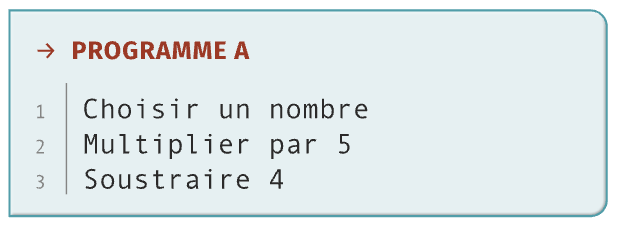
\includegraphics[width=0.46\textwidth]{programme-A.png}\hspace{0.03\textwidth}%
    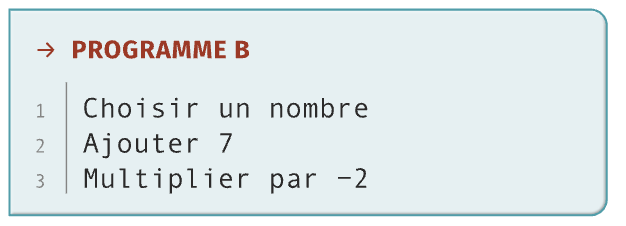
\includegraphics[width=0.46\textwidth]{programme-B.png}
  \end{center}

  \begin{enumerate}[label=\alph*)]
    \item On note $x$ le nombre choisi au départ. Exprimer en fonction de $x$ le résultat
          de chaque programme, puis écrire l'équation traduisant que les deux programmes
          donnent le même résultat.
    \item Résoudre cette équation.
  \end{enumerate}
\end{enumerate}

%================= FONCTIONS =================

\exo{Fonctions linéaires et affines}
\begin{enumerate}
  \item Soit $f$ la fonction linéaire définie par :

  \vspace{5pt}
  \hspace{1cm} $f(x) = 3x$

  \vspace{5pt}
  Calculer $f(2)$ et $f(-4)$, puis déterminer l'antécédent de $21$ par $f$.
  \item Soit $g$ la fonction affine définie par :

  \vspace{5pt}
  \hspace{1cm} $g(x) = -2x + 5$

  \vspace{5pt}
  Calculer $g(0)$ et $g(3)$, puis résoudre $g(x) = 0$.
  \item Pour la fonction $g$ ci-dessus, préciser son coefficient directeur et son ordonnée à l'origine.
  \item Déterminer l'expression de la fonction affine $h$ telle que :

  \vspace{5pt}
  \hspace{1cm} $h(0) = 1$ \qquad \qquad $h(4) = 9$
\end{enumerate}

\end{document}
